\documentclass{article}
% translate with >> pdflatex -shell-escape <file>

% This file is used as unit test for pgfplots, copyright by Christian Feuersaenger.
% 
% See
%   http://pgfplots.sourceforge.net/pgfplots.pdf
% for pgfplots.
%
% Any required input files (for <plot table> or <plot file> or the table package) can be downloaded
% at
% http://www.ctan.org/tex-archive/graphics/pgf/contrib/pgfplots/doc/latex/
% and
% http://www.ctan.org/tex-archive/graphics/pgf/contrib/pgfplots/doc/latex/plotdata/

\usepackage{pgfplots}
\pgfplotsset{compat=newest}

\pagestyle{empty}

\begin{document}
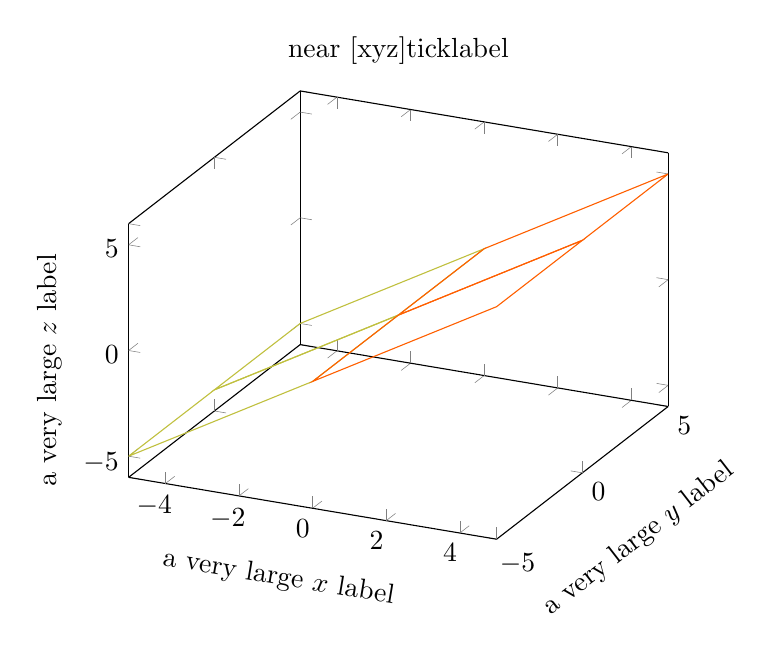
\begin{tikzpicture}
		\begin{axis}[
			title={near [xyz]ticklabel},
			xlabel=a very large $x$ label,
			ylabel=a very large $y$ label,
			zlabel=a very large $z$ label,
			label style={sloped},
		]
		
		\addplot3[mesh,samples=3] {x};
		\end{axis}
	\end{tikzpicture}
\end{document}
